%\documentclass[12pt,a4paper]{article}
\documentclass[german,bibnum,beleg,zihtitle,german,hyperref,utf8]{zihpub}
\author{\begin{tabular}{cc}
Maximilian Knespel & 3803449 \\
Moritz Häussler & 4096912 \\
Korcan Kirikici & 4049055
\end{tabular}
}
\betreuer{Nico Hoffmann}
\title{Hauptseminar}
\date{}
\bibfiles{literatur}

\usepackage[utf8]{inputenc}
\usepackage[T1]{fontenc}
	% if you don't use \usepackage[T1]{fontenc},
    % - Words containing accented characters (ö,...) cannot be automatically hyphenated,
    % - You cannot properly copy-and-paste srom the output (DVI/PS/PDF),
    % - Characters like the pipe sign, less than and greater sign give unexpected results in text.
\usepackage{lmodern}  % Vector Fonts even when using T1 !
%\usepackage[ngerman]{babel}
\usepackage[dvipsnames,cmyk,table]{xcolor} % xcolor and more colornames, cymk for printing
\usepackage{cmap} % pro­vides char­ac­ter map ta­bles, which makes PDFs search­able and copy-able (I don't see a difference yet!!!)
\usepackage[labelfont=bf,format=plain]{caption} % allows captions in non-figure environments with \captionof and \captionsetup
\usepackage[binary-units=true]{siunitx}    % SI units paper conform with \SI{3}{\nano\seconds}
\usepackage{tabularx}
\newcolumntype{Y}{>{\centering\arraybackslash}X}

\definecolor{mygreen}{rgb}{0,0.6,0}
\definecolor{mygray}{rgb}{0.5,0.5,0.5}
\definecolor{mymauve}{rgb}{0.58,0,0.82}

\usepackage{listings}   % source code listings
\usepackage{textcomp}
\usepackage{courier}
\usepackage{float}      % enables \begin{figure}[H] to disable floating figure
\usepackage{ulem}

\lstset{ %
  backgroundcolor=\color{white},   % choose the background color; you must add \usepackage{color} or \usepackage{xcolor}
  basicstyle=\footnotesize\ttfamily, % the size of the fonts that are used for the code
  breakatwhitespace=false,         % sets if automatic breaks should only happen at whitespace
  breaklines=true,                 % sets automatic line breaking
  captionpos=b,                    % sets the caption-position to bottom
  commentstyle=\color{mygreen},    % comment style
%  deletekeywords={...},            % if you want to delete keywords from the given language
  escapeinside={\%*}{*)},          % if you want to add LaTeX within your code
  extendedchars=false,              % lets you use non-ASCII characters; for 8-bits encodings only, does not work with UTF-8
  %frame=single,                    % adds a frame around the code
  keepspaces=true,                 % keeps spaces in text, useful for keeping indentation of code (possibly needs columns=flexible)
  keywordstyle=\color{blue},       % keyword style
  morekeywords={*,...},            % if you want to add more keywords to the set
  numbers=left,                    % where to put the line-numbers; possible values are (none, left, right)
  numbersep=5pt,                   % how far the line-numbers are from the code
  numberstyle=\tiny\color{mygray}, % the style that is used for the line-numbers
  rulecolor=\color{black},         % if not set, the frame-color may be changed on line-breaks within not-black text (e.g. comments (green here))
  showspaces=false,                % show spaces everywhere adding particular underscores; it overrides 'showstringspaces'
  showstringspaces=false,          % underline spaces within strings only
  showtabs=false,                  % show tabs within strings adding particular underscores
  stepnumber=1,                    % the step between two line-numbers. If it's 1, each line will be numbered
  stringstyle=\color{mymauve},     % string literal style
  tabsize=2,                       % sets default tabsize to 2 spaces
  title=\lstname,                  % show the filename of files included with \lstinputlisting; also try caption instead of title
  xleftmargin=.25in,               % indent listings by default
  upquote=true                     % single quotes '' appear straight instead of as backticks. Needs textcomp
}

\usepackage{amsmath, amsthm, amssymb}
\allowdisplaybreaks
\setlength\parindent{0pt} % stop indenting every paragraph by 1cm. It looks awful!
\usepackage{esint} % for oiint
\usepackage{attachfile} % insert attachments into pdf O_O

%\usepackage{pdfpages}   % include single pages from larger pdfs (this is a pdfxcviewerpro feature, it's cool that latex can do this for free!!)

\usepackage{enumitem}
\setitemize{itemsep=0pt,topsep=3pt}
\setenumerate{itemsep=0pt,topsep=3pt}

% http://tex.stackexchange.com/questions/2644/how-to-prevent-a-page-break-before-an-itemize-list
\makeatletter
\newcommand{\nolisttopbreak}{\vspace{\topsep}\nobreak\@afterheading}
\makeatother


%%%%%%%%%%%%%%%%%%%%%%%%%%%%%%%%%%%%%%%%%%%%%%%%%%%%%%%%%%%%%%%%%%%%%%%%%%%%%%%%
% main part
%%%%%%%%%%%%%%%%%%%%%%%%%%%%%%%%%%%%%%%%%%%%%%%%%%%%%%%%%%%%%%%%%%%%%%%%%%%%%%%%

\begin{document}

\hyphenchar\font=\string"7F % make "= unneeded
%\hyphenation{Kon-fi-gu-ra-ti-ons-tool} % why isn't this working damn it!?

% All files must be UTF8-without BOM encoded!!!

%sed -e 's/\\section/\\chapter/'          -i Aufgabe*.tex
%sed -e 's/\\subsection/\\section/'       -i Aufgabe*.tex
%sed -e 's/\\subsubsection/\\subsection/' -i Aufgabe*.tex

\chapter{Einführung}
Im Rahmen dieser Belegarbeit soll ein Ansatz entwickelt werden, um in Java oder Scala auf Clustern auf Grafikkarten zu berechnen. Es wurde sich für eine Kombination von Spark für die Kommunikation im Cluster und Rootbeer für die Grafikkartenprogrammierung entschieden.

Zuerst wird in den Kapiteln \ref{sct:montecarloalgo}-\ref{sct:spark} die benutzten Algorithmen und Bibliotheken vorgestellt, in Kapitel~\ref{sct:implementation} wird die eigene Implementierung dokumentiert und in Kapitel~\ref{sct:benchmarks} werden Benchmarks dieser Implementierung vorgestellt.

%Dabei soll die Vorgehensweise reproduzierbar dokumentiert werden, mit dem Ziel, die Programmierung auf Grafikkarten-Clustern so einfach wie möglich zu machen. Z.B. durch ein Skript. Als ersten Testfall wird ein Monte-Carlo-Algorithmus zur Berechnung von Pi implementiert, da dieser sehr rechenlastig ist. Weiterhin soll ein kommunikationslastiger Algorithmus wie z.B. Mergesort auf einem Grafikkartencluster untersucht werden.

\chapter{Rechenintensiver Testalgorithmus}
\label{sct:montecarloalgo}

\section{Monte-Carlo Algorithmen}

Monte-Carlo-Algorithmen bezeichnet Algorithmen, die mit Hilfe von (Pseudo-)Zufallszahlen versuchen das gesuchte Ergebnis statistisch zu approximieren. Dafür werden Stichproben aus statistischen Verteilungen durch z.B. physkalisch begründete Abbildungen transformiert und jene Ergebnisse statistisch ausgewertet. Diese Art von Verfahren eignet sich z.B. zur Berechnung von Integralen über zig Koordinaten, die mit üblichen Newton-Cotes-Formeln aufgrund der hohen Dimensionalität nicht praktikabel wären. Eine andere Anwendung ist die Analyse von durch kosmischer Strahlung ausgelösten Teilchenschauern mit Hilfe von Markov-Ketten\cite{metropolis1949monte}.

Monte-Carlo-Algorithmen sind als statistische Stichprobenverfahren schon länger bekannt, wurden aber erst mit dem Aufkommen der ersten Computer, z.B. dem ENIAC um 1947-1949, praktikabel\cite{metropolis1987beginning}. Der Name, nach der Spielbank ''Monte-Carlo'', wurde von N.Metropolis vorgeschlagen und hielt sich seitdem. Der Vorschlag zu dieser Art von Algorithmus kam von John von Neumann auf, als man mit dem ENIAC thermonukleare Reaktionen simulieren wollte. Aber Fermi wird nachgesagt schon Jahre zuvor statistische Stichprobenverfahren in schaflosen Nächten händisch angewandt zu haben und mit den überraschend genauen Resultaten seine Kollegen in Staunen zu versetzen.

Monte-Carlo-Verfahren sind inhärent leicht zu parallelisieren, da eine Operation, die Simulation, mehrere Tausend oder Milliarden Mal ausgeführt wird. Eine Schwierigkeit besteht jedoch darin den Pseudozufallszahlengenerator (pseudorandom number generator - PRNG) korrekt zu parallelisieren. Das heißt vor allem muss man unabhängige Startwerte finden und an die parallelen Prozesse verteilen.
 - Zeitangaben sind hierbei nicht sinnvoll. Das betrifft alle möglichen Zeitgeber in Rechnern wie z.B. .

\subsection{Berechnung von Pi}

Um Pi zu berechnen wird Pi als Integral dargestellt, da sich beschränkte Integrale durch Monte-Carlo-Verfahren approximieren lassen.
\begin{equation}
	\pi = \int \begin{cases}
					1 & |x^2+y^2| \leq 1\\
					0 & \text{sonst} 
			   \end{cases} 
		  \mathrm{d}x \mathrm{d}y
\end{equation}
Das heißt wir integrieren die Fläche eines Einheitskreises. Durch die Ungleichung wissen wir auch, dass nur für $x,y\in [-1,1]$ der Integrand ungleich $0$ ist. 

Da es programmatisch trivialer ist Zufallszahlen aus dem Intervall $[0,1]$ anstatt $[-1,1]$ zu ziehen, wird das Integral über den Einheitskreis in ein Integral über einen Viertelkreis geändert:
\begin{equation}
	\label{eq:piint}
	\pi = 4 \int\limits_{0}^\infty \mathrm{d}x  
		    \int\limits_{0}^\infty \mathrm{d}y 
		    \begin{cases}1 & |x^2+y^2| \leq 1\\0 & \text{sonst} \end{cases}
\end{equation}

Das Vorgehen ist nun wie folgt
\begin{enumerate}
	\item Setze die Zählvariable \texttt{Summe} auf $0$
	\item Ziehe für $x$ und $y$ je eine gleichverteilte Zufallszahl aus dem Intervall $[0,1]$\ 
	\item Falls $x^2+y^2<1$, dann erhöhe \texttt{Summe} um $1$
	\item Gehe zu 2.
\end{enumerate}
Mathematisch ausgedrückt also:
\begin{equation}
	\label{eq:pimonteint}
	\mu_N = \langle f\left( \vec{x}_i \right) \rangle := \frac{1}{N} \sum_{i=1}^N f\left( \vec{x}_i \right),\;\vec{x}_i \text{ uniform zufallsverteilt aus } \Omega:=[0,1]\times[0,1]
\end{equation}
Im allgemein ist $f$ eine beliebige Funktion, aber für die Berechnung von Pi ist es die Einheitskugel in 2D, vgl.Gl.\ref{eq:piint}.

In Python kann man dies, wenn man sich auf Einkernprozessoren einschränkt, mit NumPy\cite{numpy} in nur wenigen zeilen niederschreiben:
\begin{lstlisting}[language=python]
from numpy import *
N=10000000
x=random.rand(N)
y=random.rand(N)
pi = 4.0 * sum( x*x + y*y < 1 ) / N
\end{lstlisting}\vspace{-1.5\baselineskip}

Der Vollständigkeit halber seien kurz ein paar Worte zu den Rändern verloren, das betrifft die Zufallszahlen die entweder aus einem rechtsoffenem oder geschlossenen Intervall $[0,1]$ stammen können und den Vergleich, der die Gleichheit mit einschließen kann oder nicht.

Aus der Integraltheorie ist klar, dass die Ränder ein Nullmaß haben und damit keine Rolle spielen. Aber für diskrete Verfahren könnte dies zu einer zusätzlichen systematischen Fehlerquelle führen, der Fehlerskalierverhalten möglicherweise beeinträchtigt.

Am Beispiel von nur vier Zuständen für Zufallszahlen für den rechtsoffenen Fall, also $x,y\in \lbrace 0,0.25,0.5,0.75 \rbrace$, sei dies einmal durchgedacht. Damit ergibt sich
\begin{equation}
	x^2+y^2 = \lbrace 0, 0.0625, 0.125, 0.25, 0.3125, 0.5, 0.5625, 0.625, 0.8125, 1.125 \rbrace
\end{equation}
% (Python-Skript für Kombinationen:
%    x=array([0,1,2,3])/4.
%    a,b=meshgrid(x**2,x**2)
%    unique( (a+b).ravel() )
Hier macht es aufgrund der begrenzten Anzahl an Zuständen, unter denen die $1.0$ ohnehin nicht auftritt, keinen Unterschied ob man $<$ oder $\leq$ vergleicht, man erhielte Pi zu $3.6$.
Hinzu kommt aber, dass Zustände auf den Grenzen $x=0$ und $y=0$ liegen, sodass die Grenzen vierfach gezählt werden da wir nur den Viertelkreis berechnen und mit vier multiplizieren. 

Man hat also ohnehin immer einen Diskretisierungsfehler von $O\Delta x)$ wobei $\Delta x$ die Diskretisierungslänge zwischen zwei Zuständen ist. Angemerkt sei, dass dies für Gleitkommazahlen komplizierter gestaltet.

Abschließend sei angemerkt, dass Monte-Carlo-Methoden dafür gedacht sind einen praktisch unerschöpflichen Raum Stichprobenartig auszutesten, sodass Diskretisierungs- und Randfehler ohnehin als vernachlässigbar angenommen werden. Wenn man merkt, dass es zu Diskretisierungsfehler wie obig an den Rändern kommt, oder man gar die Anzahl aller möglichen Zustände an Zufallszahlen erschöpft hat und sich die Approximation damit nicht mehr verbessern kann, sollte man über ein anderes Verfahren nachdenken oder den Zufallsgenerator anpassen und z.B. mit 128-Bit statt 32-Bit betreiben. Auch die maximale Periodenlänge von Pseudozufallsgeneratoren spielt hier eine Rolle!
%
%Mit geschlossenen Grenzen hingegen wären $x,y\in\lbrace 0,\frac{1}{3},\frac{2}{3},1 \Rightarrow \rbrace 0, \frac{1}{9}, \frac{2}{9}, \frac{4}{9}, \frac{5}{9}, \frac{8}{9}, 1 \frac{10}{9}, \frac{13}{9},2 \rbrace$
% Man beachte, dass float ohnehin nur 32 Bit ist, wovon 1 bit das Vorzeichen und 8 bit der Exponent ist. Da wir uns immer nur im Intervall [0,1] befinden nutzen wir Vorzeichen und Exponent ohnehin nicht, sodass nur 23 Bit Präzision benutzt werden. Das sind also nur 2^23 \approx 10^7 erreichbare Zustände. Moderne Prozessoren können leicht 10^9 Operationen pro Sekunde rechnen, sodass einfache Fließkommagenauigkeit nicht ausreicht, da schon nach einigen Millionen Stichproben sich der relative Fehler nicht mehr verbessern, aber auch nciht mehr verschlechtern, wird. Siehe dazu Abb.\ref{fig:monteerrorfloat}

Da die Monte-Carlo-Pi-Integration einer Mittelwertbildung entspricht, vgl. Gl.\ref{eq:pimonteint}, ist die statistische Unsicherheit gegeben durch die Standardabweichung des Mittelwerts $\sigma_{\mu_N}$, welche gegeben ist als
\begin{equation}
	\sigma_{\mu_N} \frac{\sigma}{\sqrt{N}}
\end{equation}
wobei $\sigma$ die Standardabweichung der Stichprobe ist, vgl. Anhang~\ref{apx:meanerror}.
Wenn $f_i$ in einem beschränkten Intervall liegt, dann ist auch die Standardabweichung der Stichproben $f_i$ beschränkt, sodass die Standardabweichung auf den Mittelwert $\propto \frac{1}{\sqrt{N}}$ abnimmt.

\begin{figure}
	\centering
	\begin{minipage}{0.7\linewidth}
		\includegraphics[width=\linewidth]{monte-carlo-pi-error-scaling}
	\end{minipage}
	\caption{captiontext}
	\label{fig:monteerrorfloat}
\end{figure}


\subsection{Pseudozufallszahlgeneratoren}


\section{Vergleich - Alternativen}


\chapter{Rootbeer}
\label{sct:rootbeer}

Rootbeer\cite{pratt2012rootbeer} ist ein von Philip C. Pratt-Szeliga entwickeltes Programm und Bibliothek welches das Schreiben von CUDA-Kerneln in Java erleichtert. Zum aktuellen Zeitpunkt Mai 2016 hat Rootbeer leider noch Beta-Status und wurde seit ca. einem Jahr nicht weiterentwickelt\cite{rootbeergithub}.

Mit Rootbeer lassen sich CUDA-Kernel direkt in Java schreiben anstatt in C/C++. Dafür muss zuerst vom Nutzer die \texttt{org.trifort.rootbeer.runtime.Kernel}-Klasse implementiert und zu einer Java class-Datei kompiliert werden. 
Wenn das komplette zu schreibende Programm zu einer jar-Datei zusammengefügt wurde, dann muss diese noch einmal an den Rootber-Compiler übergeben werden. Rootbeer nutzt Soot\cite{sootsite,sootretrospective}, um den Bytecode in Jimple zu übersetzen. Jimple ist eine vereinfachte Zwischendarstellung von Java-Bytecode, welcher ca. 200 verschiedene Befehle besitzt, in Drei-Address-Code mit nur 15 Befehlen.
Der Jimple-Code wird dann analysiert und in CUDA übersetzt welcher dann mit einem installierten NVIDIA-Compiler übersetzt wird. All das geschieht automatisch, aber die Zwischenschritte kann man zur Fehlersuche unter Linux in \lstinline!$HOME/.rootbeer/! einsehen.
Die erstellte cubin-Datei wird zusammen mit \texttt{Rootbeer.jar} der jar-Datei des selbstgeschriebenen Programms hinzugefügt.

Die zweite große Vereinfachung, die Rootbeer zur Verfügung stellt, ist die Automatisierung des Datentransfers zwischen GPU und CPU. Das besondere hierbei ist, dass Rootbeer die Nutzung von beliebigen, also insbesonderen auch nicht-primitiven Datentypen erlaubt. Diese Datentypen serialisiert Rootbeer automatisch und unter Nutzung aller CPU-Kerne und transferiert sie danach auf die Grafikkarte.

Diese zwei Vereinfachungen obig machen die erste Nutzung von Rootbeer verglichen zu anderen Lösungen sehr einfach, sodass Rootbeer insbesondere für das Erstellen von Prototypen günstig ist.
In Kontrast dazu ist es jedoch auch mögliche wiederum sehr nah an der Grafikkarte zu programmieren. Dafür kann man mit Rootbeer auch manuell die Kernel-Konfiguration angeben, mehrere GPUs ansprechen und auch shared memory nutzen.

\section{Nutzung}

Für die Nutzung von Rootbeer unter Debian-Derivaten ist das \texttt{openjdk-7-jdk}-Pakt und das \texttt{nvidia-cuda-toolkit}-Paket notwendig. Leider funktioniert Rootbeer nicht mit JDK 8. JDK 7 funktioniert vollends in den hier durchgeführten Beispielen, aber volle Unterstützung ist bisher nur für JDK 6 offiziell gegeben\cite{rootbeerjdk6}.

Ein Minimalbeispiel für einen Kernel, dessen Threads nur ihre ID in einen Array schreiben sieht wie folgt aus:
\lstinputlisting[language=Java]{minimal/ThreadIDsKernel.java}
Der Aufruf der Kernels geschieht über eine Liste von Kernel-Objekten, die per Konstruktor mit Parametern initialisiert wurden. Diese Liste wird an \texttt{rootbeer.run} übergeben, der den Kernel dann mit einer passenden Konfiguration startet.
\lstinputlisting[language=Java]{minimal/ThreadIDs.java}
Zuerst müssen diese beiden Dateien mit `javac` kompiliert werden und dann zusammen mit einer `manifest.txt`-Datei, die die Einsprungsklasse anzeigt, zu einem Java-Archiv gepackt werden, welches im letzten Schritt mit Rootbeer kompiliert und dann ausgeführt wird.
\lstinputlisting[language=Bash]{minimal/compile.sh}
Bei der Kompilierung mit \texttt{Rootbeer.jar} muss beachtet werden, dass alle benutzten Klassen mit in der jar-Datei enthalten sind, sonst quittiert Soot mit folgender Fehlermeldung:
\begin{lstlisting}
java.lang.RuntimeException: cannot get resident body for phantom class
\end{lstlisting}\vspace{-1.5\baselineskip}
Bei Nutzung von scala heißt das insbesondere, dass \texttt{scala.jar} mit in das Java-Archiv gepackt werden muss.

Weiterhin ist zu beachten, dass die an Rootbeer/Soot übergebene Datei entgegen der Linux-Ideologie mit \texttt{.jar} enden muss, insbesondere führen Dateinamen wie \texttt{gpu.jar.tmp} zu der Fehlermeldung 
\begin{lstlisting}
There are no kernel classes. Please implement the following interface to use rootbeer:
org.trifort.runtime.Kernel
\end{lstlisting}


\section{Multithreaded Rootbeer}

Bei der Benutzung von Rootbeer, kam es leider zu einigen Bugs, die teilweise in einem geforkten Repository auf Github behoben wurden, siehe~\cite{ownrootbeerfork}.
Das wichtigste Problem sei hier kurz vorgestellt.

Auf Taurus ist das Heimverzeichnis über alle Knoten zugreifbar. Dies führt zu einen Problem, wenn man Rootbeer auf verschiedenen Nodes oder von verschiedenen Threads aus nutzen möchte, da bei einem Kernel-Aufruf \lstinline!~/.rootbeer/rootbeer_cuda_x64.so.1! aus der jar-Datei extrahiert wird. Wenn also ein Thread meint die Datei fertig entpackt zu haben, während ein anderer Thread die Datei nochmal entpackt, aber noch nicht fertig ist, dann kam es in ersten Versuchen zu einem \texttt{java.lang.UnsatisfiedLinkError}. Dies wurde behoben, indem ein Pfad aus Hostname, Prozess-ID und Datum genutzt wird:
\begin{lstlisting}[language=Java]
m_rootbeerhome = home + File.separator + ".rootbeer" + File.separator
               + getHostname() + File.separator
               + getProcessId("pid") + "-" + System.nanoTime()
               + File.separator;
\end{lstlisting}\vspace{-1.5\baselineskip}
Dies resultiert z.B. in diesen Pfad: \lstinline!~/.rootbeer/taurusi2093/7227-311934180383710/!.
%Hier ist jedoch zu beachten, dass diese extrahierten Dateien bei Programmablauf nicht automatisch gelöscht werden.


\chapter{Scala}
\label{sct:scala}

\section{Kurzbeschreibung}

\section{Funktionsweise}

\section{Anwendung}

\section{Probleme}
Counting Variable ..

\chapter{Spark}
\label{sct:spark}

% Zusammenfasung
Spark ist ein Programmierframework für Datenanalyse auf Clustern, was vor allem zusammen mit dem Stichwort Big-Data und maschinellem Lernen an Beliebtheit gewonnen hat. Es vereinigt hierbei ausfallgehärtet Funktionalitäten von Batchverarbeitungssystem bzw. Cluster-Management wie Slurm, paralleler Kommunikation zwischen Prozessen wie OpenMPI und OpenMP und Programmierbibliotheken. Die von Spark zur Verfügung gestellten primitiven sind inhärent hochparallel und ausfallgehärtet ausführbar und aus Java, Scala und Python heraus ansprechbar. Aus letzteren beiden auch interaktiv, was das Experimentieren und schnelle Erstellen von Prototypen vereinfacht. Es gibt erweiternde Bibliotheken für maschinelles Lernen und Graphen. Der große Funktionsumfang macht es für Anfänger schwer einzuordnen, was Spark ist, aber ermöglich das schnelle interaktive und nichtinteraktive Auswerten von Big Data auf Clustern.

% Kurze Entstehungsgeschichte, um das alles einordnen zu können, Zusammenhang mit Map-Reduce-Paradigma
%Spark wurde an der Berekely Universität entwickelt. (in memory. Spark erweitert das Map-Reduce-Paradigma mit komplexeren Operationen, sodass man ein Problem nicht mehr auf Map-Reduce konvertieren muss. Spark kann benutzt werden von Python, Java, Scala und SQL.
%
%Eine Map ist eine Abbildung die einem Eingabewert einen Ausgabewert zuordnet. Im Zusammenhang mit paralleler Programmierung bezeichnet sie ein Programmiermuster für trivial parallelisierbare Probleme, das heißt solche, die keine Kommunikation untereinander erfordern. Ein Beispiel sind mit OpenMP  \lstinline!#pragma omp parallel for! parallelisierte Schleifen. Jede Schleifeiteration kann dabei als eine Abbildung ohne Kommunikation angesehen werden.
%
%Eine Reduce-Operation ist 
%
% - spark vereinfacht mapReduce programmierung, keine manuelle Zerelegung in batche jobs mehr nötig
% - Mischung aus OpenMPI, Slurm und Programmierparadigma
% - sehr beliebt in Machine Learning

\section{Konfiguration von Spark auf Taurus}

Um Spark nutzen zu können müssen zuerst Master- und Slave-Knoten gestartet werden. Hier soll es nur einen Master-Knoten und $n$ Slave-Knoten geben. Damit alle gleichzeitig gestartet werden, kann Slurms \lstinline!--multi-prog! Option genutzt werden, welche als Argument einen Pfad zu einer Konfigurationsdatei erwartet, in der für jeden Rank ein auszuführendes Programm angegeben werden muss.

Alternativ kann man auch anhand von der Umgebungsvariable \lstinline!SLURM_PROCID! im Skript entweder einen Master-Knoten oder einen Slave-Knoten starten. Letzeres wurde aufgrund der Übersichtlichkeit, d.h. alle Funktionalitäten in einem Skript zu haben, gewählt, siehe Listing~\ref{lst:start_spark_slurm.sh}.

Wenn Spark gestartet ist, kann sich z.B. mit einer aktiven Eingabeaufforderung an den Master verbunden werden:
\begin{lstlisting}[language=bash]
spark-shell --master=$MASTER_ADDRESS
\end{lstlisting}\vspace{-1.5\baselineskip}


\chapter{Eigene Implementierung}
\label{sct:implementation}

\section{Kompilierung}

%Versucht man mit \lstinline!Rootbeer.jar! eine jar-Datei, welche auch Scala-Klassen beinhaltet, in GPU-Code umsetzen zu lassen, z.B. auf diese Weise:
%
%\begin{lstlisting}[language=bash]
%scalac $< -classpath $(ROOTBEER_ROOT)/Rootbeer.jar:. -deprecation
%javac $< -classpath $(ROOTBEER_ROOT)/Rootbeer.jar:.
%scalac $< -classpath $(ROOTBEER_ROOT)/Rootbeer.jar:. -deprecation
%jar -cvfm MontePiGPU.jar.tmp.jar manifest.txt *.class
%java -jar Rootbeer.jar MontePiGPU.jar.tmp.jar MontePiGPU.jar -64bit -computecapability=sm_30
%\end{lstlisting}
%
%Dann kommt es bei soot zu einer Runtime Exception:
%
%\begin{lstlisting}
%java.lang.RuntimeException: cannot get resident body for phantom class : <MonteCarloPiKernel$$anonfun$gpuMethod$1: void <init>(MonteCarloPiKernel,scala.runtime.ObjectRef)>; maybe you want to call c.setApplicationClass() on this class!
%	at soot.SootMethod.retrieveActiveBody(SootMethod.java:316)
%	at soot.rbclassload.RootbeerClassLoader.loadScene(RootbeerClassLoader.java:857)
%	at soot.rbclassload.RootbeerClassLoader.loadNecessaryClasses(RootbeerClassLoader.java:320)
%	at org.trifort.rootbeer.entry.RootbeerCompiler.setupSoot(RootbeerCompiler.java:198)
%	at org.trifort.rootbeer.entry.RootbeerCompiler.compile(RootbeerCompiler.java:219)
%	at org.trifort.rootbeer.entry.RootbeerCompiler.compile(RootbeerCompiler.java:213)
%	at org.trifort.rootbeer.entry.Main.run(Main.java:208)
%	at org.trifort.rootbeer.entry.Main.main(Main.java:244)
%\end{lstlisting}
%
%"Phantom classes are implicitly created models of classes that do not exist on Soot's classpath. To get rid of this problem, make sure that the class you are referencing is on Soot's classpath." \url{http://stackoverflow.com/questions/27383832/why-is-soot-always-saying-that-the-class-i-want-to-load-is-a-phantom-class-even}
%
%Nachdem nun also \lstinline!spark-library.jar! hinzugefügt wurde, verschwindet diese exception, aber Rootbeer findet die Kernel-Implementierung nicht:
%\begin{lstlisting}
%There are no kernel classes. Please implement the following interface to use rootbeer:
%org.trifort.runtime.Kernel
%\end{lstlisting}
%
%Dies könnte daran liegen, das \lstinline!MonteCarloPiKernel.scala! scala benutzt. Dadurch wird für \texttt{soot} verschleiert, dass die Klasse \texttt{Kernel} implementiert.
%Eine Implementierung in java löst das Problem jedoch nicht. Vermutlich weil \texttt{soot} oder \texttt{Rootbeer} nur Klassen analysieren die von der main-Klasse aufgerufen werden. Da die  main-Klasse aber in scala geschrieben ist, ist der Aufruf womöglich für \texttt{soot} nicht sichtbar, sodass \texttt{soot} \texttt{MonteCarloPiKernel.class} als unbenutzt einstuft und ignoriert. Ein Hinweis darauf liefert diese Ausgabe von Soot bei der Ausführung von Rootbeer:
%\begin{lstlisting}
%Total loaded classes: 557
%Total loaded methods: 0
%\end{lstlisting}
%Bei der Java-Version funktioniert die Kompilierung mit Rootbeer und die Ausgabe ist:
%\begin{lstlisting}
%Total loaded classes: 1428
%Total loaded methods: 4385
%\end{lstlisting}
%Eine mögliche Lösung wäre es eine Dummy-Java-Klasse zu schreiben die alle Kernel-Implementierungen aufruft und als main-class im Manifest festgelegt ist. 
%Das Problem hierbei ist jedoch, dass Rootbeer Serialisierungs- und Deserialisierungscode in die aufrufende Klasse injeziert. Damit dieser injezierte Code also nicht in die Dummy-Klasse eingesetzt wird, braucht es noch eine Wrapper-Klasse, welche die Kernel-Implementierung aufruft und von der Dummy-Klasse aufgerufen wird. Dies ist \texttt{MonteCarloPi.java}.
%
%Nachdem die Kompilierung mit \texttt{Rootbeer} dann erfolgt ist, muss die Manifest-Datei \texttt{META-INF/MANIFEST.MF} dann nur noch abgeändert werden, damit sie nicht mehr auf die Dummy-Klasse verweist. Durchgeführt wurde es ähnlich, jedoch wurden alle nicht für Rootbeer relevanten Klassen erst nach dem Rootbeer-Aufruf zusammen mit der neuen Manifest-Datei in eine jar-Datei zusammengeführt, siehe Abb.\ref{fig:compilation}.


\begin{figure}[H]
	\centering
	\begin{minipage}{\linewidth}
		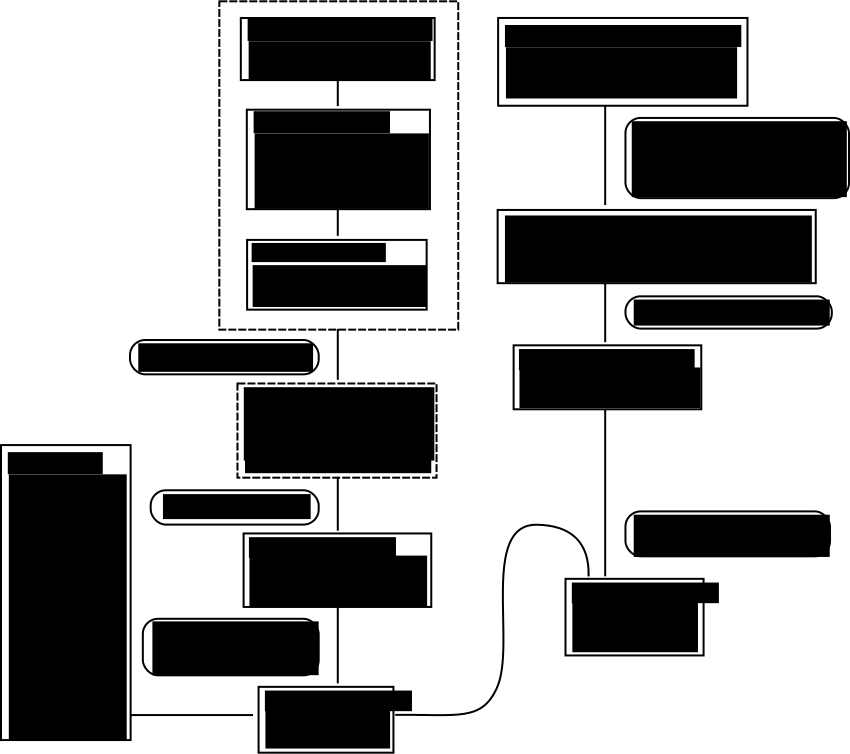
\includegraphics[width=\linewidth]{compile-structure-deu.pdf}
	\end{minipage}
	\caption{Kompilationsschema mit Kommadozeilenbefehlen und Zwischenstati.}
	\label{fig:compilation}
\end{figure}

!!! Problem: Hab mehrere Fehler gefunden deren Kenntnis möglicherweise eine Vereinfachung des Schemas bedeutet. Da bin ich noch am rumspielen, daher ist das halbfertig.

\section{Probleme}
Implementierung:
    Was ist bei GPUs zu beachten ( Seeds, 64-Bit )
    Was ist bei Rootbeer zu beachten?
      - private Variablen werden wirklich immer per memcpy hin und her transportiert.
      - muss nicht auf ungerade Kernel-Zahl achten, werden automatisch aussortiert


\chapter{Benchmarks}
\label{sct:benchmarks}

\section{Testsysteme}
\subsection{System 1: Heimsystem}
\label{sct:system1}

Aufgrund der leichten Verfügbarkeit und als Beispiel für Grafikkartenbeschleuniger im nicht-professionellen Verbrauchersegment, wurden einige Tests auf einem herkömmlichen Arbeitsplatzrechner ausgeführt:

\begin{table}[H]
	\begin{center}\begin{tabularx}{0.9\linewidth}{r|X}
	Prozessor & Intel(R) Core(TM) i3-3220 (Ivy-Bridge), \SI{3.30}{\giga\hertz}, 2 Kerne (4 durch SMT), AVX\cite{ark3220} \\
	Arbeitsspeicher & $4\times \SI{4}{\gibi\byte}$ DDR3 \SI{1600}{\mega\hertz} CL9\cite{corsair4gbddr3}\\
	\hline
	Grafikkarte & GigaByte GTX 760 WindForce 3X Overclocked, Codename: GK104-225-A2 (Kepler), 1152 CUDA-Kerne, \SI{1085}{\mega\hertz} ( \SI{1150}{\mega\hertz} Boost), \SI{2}{\gibi\byte} GDDR5-VRAM mit \SI{1502}{\mega\hertz} PCIe-3.0-x16-Schnittstelle\cite{gigabytegtx760,gtx760,nvidiakepler}
	\end{tabularx}\end{center}
	\caption{Heimsystemkonfiguration}
\end{table}

Die Maximalleistung in der Berechnung von Fließkommazahlen einfacher Genauigkeit (SPFLO) im Verhältnis einer Multiplikation zu einer Addition beträgt
\begin{align}
	\SI{3.30}{\giga\hertz} \cdot
	2\,\text{Kerne} \left( 
		1\,\frac{ \text{AVX ADD Einheit} }{ \text{Kern} } + 
		1\,\frac{ \text{AVX MUL Einheit} }{ \text{Kern} } 
	\right) \cdot
	8\,\frac{ \text{SPFLO} }{ \text{AVX Einheit} } \\ 
	= 105.6\,\text{GSPFLOPS}
\end{align}
für den Prozessor. Informationen zur Architektur, wie die Anzahl an AVX-Einheiten wurde aus Ref.\cite{cesga} entnommen.

Die Maximalleistung der Grafikkarte beträgt:
\begin{align}
	\SI{1.085}{\giga\hertz} \cdot 1152 \text{CUDA-Kerne} \cdot
	1 \frac{ \text{FMA-Einheit} }{ \text{CUDA-Kern} } \cdot
	2 \frac{ \text{SPFLO} }{ \text{FMA-Einheit} }
	= 2500\,\text{GSPFLOPS}
\end{align}
Zugegeben, es wurde beim Prozessor gespart und bei der Grafikkarte nicht, aber der Geschwindigkeitsunterschied von 24x begründet dennoch das Interesse daran Grafikkarten zu nutzen, auch wenn es bei Grafikkarten mehr zu beachten gibt, um diese Maximalleistung erhalten zu können.


\subsection{System 2: Taurus}
\label{sct:system2}

Für Skalierungstests wurde einer der Hochleistungsrechner der TU-Dresden, ein Bull HPC-Cluster mit dem Namen Taurus, benutzt. Der Bau der ersten Phase von Taurus war 2013 abgeschlossen\cite{taurusnutzerschulung}. Zum Zeitpunkt der Nutzung (2015/2016) waren alle Knoten von Phase 1 schon in die 2015 fertiggestellt\cite{heisehrsk2} Phase 2 integriert wurden\cite{doctudtaurushardware} und werden nun beide unter dem Namen Taurus zusammengefasst.

\begin{figure}[H]
	\centering
	\begin{minipage}{0.5\linewidth}
		\includegraphics[width=\linewidth]{taurusphase1}
	\end{minipage}\begin{minipage}{0.5\linewidth}
		\includegraphics[width=\linewidth]{taurusphase1island1interconnects}
	\end{minipage}
	\caption{\textbf{Links:} Übersicht Taurus Phase 1. \textbf{Rechts:} Schema der Topologie von Insel 2, auf der ausschließlich gerechnet wurde. Die Bilder wurden übernommen aus Ref.\cite{taurusnutzerschulung}}
	\label{fig:taurusphase1}
\end{figure}

Gerechnet wurde auf Insel 2 von Taurus, vgl. Tabelle~\ref{tbl:island2}. Wenn nicht anders erwähnt, dann beziehen sich Benchmarks auf die Tesla K20x Knoten.

\begin{table}[H]
	\begin{tabularx}{0.9\linewidth}{r|Y|Y}
		& \textbf{Phase 1} & \textbf{Phase 2} \\
		\hline
		Knoten          & 44 & 64 \\
		Hostnamen       & taurusi2[001-044] & taurusi2[045-108] \\
		Prozessor       & 2x Intel Xeon CPU E5-2450 (8 Kerne) @ 2.10GHz, MultiThreading deaktiviert, AVX, 2x 268.8\,GSPFLOPS
						& 2x Intel(R) Xeon(R) CPU E5-2680 v3 (12 Kerne) @ 2.50GHz, MultiThreading deaktiviertt, AVX2 insbesondere FMA3\cite{ark2680v3}, 2x 537.6\,GSPFLOPS \\
		GPU 			& 2x NVIDIA Tesla K20x & 4x NVIDIA Tesla K80 \\
		Arbeitsspeicher & \SI{32}{\gibi\byte} & \SI{64}{\gibi\byte} \\
		Festplatte      & \SI{128}{\gibi\byte} SSD & \SI{128}{\gibi\byte} SSD
	\end{tabularx}
	\caption{Zusammensetzung Insel 2 von Taurus\cite{doctudtaurussystem}}
	\label{tbl:island2}
\end{table}

\begin{table}[H]
	\begin{tabular}{r|c|c}
	& \textbf{K20x} & \textbf{K80} \\
	\hline
	Chip       & GK110 & GK210 \\
	Takt       & \SI{0.732}{\giga\hertz} & \SI{0.560}{\giga\hertz} \\
	CUDA-Kerne & 2688 & 4992 \\
	Speicher   & \SI{6}{\gibi\byte}, GDDR5 384 Bit Busbreite
	           & $2\times\SI{12}{\gibi\byte}$, GDDR5 384 Bit Busbreite \\
    Bandbreite & \SI{250}{\giga\byte\per\second}
	           & $2\times\SI{240}{\giga\byte\per\second}$              \\
%	\begin{minipage}{2.5cm}\begin{flushright}Theoretische\\Spitzenleistung\end{flushright}\end{minipage} & 3935\,GSPFLOPS, 1312\,GDPFLOPS 
%					& 5591\,GSPFLOPS, 1864\,GDPFLOPS \\
	Theoretische    & 3935\,GSPFLOPS & 5591\,GSPFLOPS \\
	Spitzenleistung & 1312\,GDPFLOPS & 1864\,GDPFLOPS
	\end{tabular}
	\caption{Spezifikationen der Kepler-Grafikkarten von Taurus\cite{nvidiakepler,k20anandtech}}
	\label{tbl:k20k80}
\end{table}

Zu den Spitzenleistungen in Tabelle~\ref{tbl:k20k80} sei angemerkt, dass jeder CUDA-Kern einfache Fließkommagenaugigkeit berechnet und auf drei CUDA-Kerne eine Doppelpräzisionseinheit kommt, wodurch sich die DFLOPS berechnen.
Die K80 hat außerdem einen Boost-Modus mit \SI{0.875}{\giga\hertz}, also einer Leistungssteigerung von $1.56$.

\section{Monte-Carlo-Simulation verschiedener Implementationen}

In Abb.\ref{fig:montepiworkloadscaling} wurde die Ausführungszeit von Monte-Carlo-Simulationen in verschiedenen Programmiersprachen über die Anzahl an Monte-Carlo-Iterationen gemessen. Gemessen wurde die Zeit mit dem Linux \texttt{time}-Befehl und zwar die \texttt{real}-Zeit. Es fällt auf, dass alle Versionen eine Initialisierungszeit haben. Bei der C++-Version beträgt diese jedoch nur knapp \SI{30}{\milli\second}, während die reine Java-Version schon ca. \SI{70}{\milli\second} benötigt. Die Nutzung von Scala erhöht dies schon auf \SI{200}{\milli\second} und die Nutzung von Rootbeer führt eine weitere Initialisierungszeit von \SI{430}{\milli\second} ein, sodass für wenig Iterationen die Rootberversion bis zu 20x langsamer sind. Erst für 10 Milliarden Iterationen beginnt die Initialisierungszeit im Vergleich zur Rechenzeit vernachlässigbar zu werden, sodass aber da die Lastenskalierung ein lineares Verhalten annimmt. Bei der C++-Version ist dies schon bei ca. 100 Millionen Iterationen der Fall.
\begin{figure}[H]
	\centering
	\begin{minipage}{0.5\linewidth}
		\includegraphics[width=\linewidth]{benchmarks-workload-scaling}
	\end{minipage}\begin{minipage}{0.5\linewidth}
		\includegraphics[width=\linewidth]{benchmarks-workload-scaling-taurus2}
	\end{minipage}
	\caption{Benötigte Ausführungszeit der Monte-Carlo Pi-Berechnung in Abhängigkeit von der Anzahl an Iterationen. Getestet auf \textbf{links:} System 1 und \textbf{rechts:} System 2 (Taurus), siehe Kapitel~\ref{sct:system1}}
	\label{fig:montepiworkloadscaling}
\end{figure}
Im Programmausdruck~\ref{lst:montemainloop} ist die Hauptschleife, die hauptsächlich die Arbeitslast generiert, zu sehen. Es handelt sich also für jede der zwei Zufallszahlen um eine Multiplikations und zwei Divisionen und dann nochmals zwei Multiplikationen für die Berechnung des Quadrat des Radius, also zusammen acht Operationen pro Iteration und neun Operationen für Iterationen die im Kreis liegen. Dies tritt für $\frac{\pi}{4}=0.785\%$ der Fälle auf, das heißt die Rechenlast, definiert als die Anzahl an arithmetischen Operationen $N_\text{Op}$ sollte sich wie folgt aus der Anzahl an Iterationen $N$ berechnen:
\begin{align}
	N_\text{Op}
	= \left[ \frac{\pi}{4}\cdot 9 + \left( 1-\frac{\pi}{4} \right)\cdot 8 \right] N
	= 8.8\cdot N
\end{align}

Zuletzt ist aus dem Plot abzulesen, dass für große Lasten wie z.B. für drei Milliarden Iterationen die Versionen, die von Grafikarten gebrauch machen, um einen Faktor $140$ (Scala) bis $320$ (C++) schneller sind als die Java Version, die auf einem Prozessor-Kern ausgeführt wird. Dieser große Unterschied zwischen CPU und GPU lässt darauf schließen, dass Java weder AVX noch mehrere Kerne gleichzeitig nutzt. Das heißt für die CPU-Versionen wäre für das Testsystem 1 noch ein Geschwindigkeitsgewinn von $8\,\frac{ \text{Op} }{ \text{AVX-Einheit} } \cdot 2\,\text{Kerne}$ erreichbar. Dies würde den Geschwindigkeitsunterschied von $320$ auf $20$ reduzieren, was in Übereinstimmung mit dem Verhältnis der Peakflops aus Kapitel~\ref{sct:system1} wäre.

\begin{lstlisting}[language=Java,caption={Hauptschleife der Monte-Carlo Pi-Berechnung},label=lst:montemainloop]
for ( int i = 0; i < dnDiceRolls; ++i )
{
    dRandomSeed = (int)( (randMagic*dRandomSeed) % randMax );
    float x = (float) dRandomSeed / randMax;
    dRandomSeed = (int)( (randMagic*dRandomSeed) % randMax );
    float y = (float) dRandomSeed / randMax;
    if ( x*x + y*y < 1.0 )
        nHits += 1;
}
\end{lstlisting}
Dieses Branching verändert also nicht das Skalierverhalten linear mit $N$, sondern führt nur zu einem veränderten Faktor. Daher ist in Abb.\ref{fig:montepiworkloadscaling} lineares Verhalten zu beobachten.

\section{Monte-Carlo-Simulation mit Spark + Rootbeer}

In Abbildung~\ref{fig:montepistrongscaling} ist die Laufzeit über die Anzahl an Kernen bzw. Grafikkarten dargestellt. Aus gründen der Rechenzeit wurde für eine Anzahl von $N=1,2,4,8,16,24,32$ Knoten die Leistungsanalyse für $4(N-1)$ bis $4N$ Kerne/Grafikkarten durchgeführt. Dies ist vor allem in der Abbildung rechts zu sehen, wo die Messpunkte immer in fünfer-Gruppen auftreten.

Zwar nicht in der Abbildung dargestellt, wurde auch für $4N+1$ und $4N+2$ gemessen. Das heißt Spark hat zwei mehr Slices zu verarbeiten als es Kerne gibt. Dies führt dazu, dass zwei Kerne doppelt so viel Arbeit wie der Rest haben, wodurch es zu einem sprunghaften Anstieg der Laufzeit kommt. Aus diesem Grund ist es normalerweise besser, wenn die Anzahl an Slices viel größer als die Anzahl an Kernen bzw. Grafikkarten wäre. Dies würde aber die ohnehin schon recht hohe Mindestproblemgröße noch einmal um ein, zwei weitere Größenordnungen erhöhen.

\begin{figure}[H]
	\centering
	\begin{minipage}{0.5\linewidth}
		\includegraphics[width=\linewidth]{cluster-strong-scaling-gpu}
	\end{minipage}\begin{minipage}{0.5\linewidth}
		\includegraphics[width=\linewidth]{cluster-strong-scaling-cpu}
	\end{minipage}
	\caption{Benötigte Ausführungszeit der Monte-Carlo Pi-Berechnung in Abhängigkeit von der Anzahl an \textbf{links:} Kernen und \textbf{rechts:} Grafikkarten. Getestet auf System 2, siehe Kapitel~\ref{sct:system2}}
	\label{fig:montepistrongscaling}
\end{figure}

Weiterhin auffällig sind zufällig auftretende Spitzen in sowohl im CPU als auch im GPU-Benchmark. Z.b. für eine Arbeitslast von $2^33$ Iterationen pro Slice auf 24 Knoten also 92 bis 96 Grafikkarten schwankt die Ausführungszeit zwischen \SI{30}{\second}, \SI{45}{\second} und \SI{68}{\second}. Möglicherweise liegt dies an einer ungünstigen Verteilugn der Slices auf die Knoten. Die vorliegende Version nimmt eine lineare Verteilung an, sodass Slice 0 auf Grafikkarte 0 von Knoten 0 rechnet, während Slice 1 auf Grafikkarte 1 von Knoten 0 und Slice 4 auf Grafikkarte 0 von Knoten 1 rechnet. Die Zeit die eine Grafikkarte für diese Last benötigt ist \SI{22}{\second}. Es ist also wahrscheinlich, dass zumindest im Fall der \SI{68}{\second} drei verschiedene Prozesse auf einem Knoten diesselbe Grafikkarte anfordern. Diese Vermutung wurde getestet, indem jeder Slice seinen Hostnamen ausgeben soll. Mit dem Skript aus Listing~\ref{lst:start_spark_slurm.sh} ist dies schnell interaktiv getestet:
\begin{lstlisting}[language=scala]
startSpark --time=04:00:00 --nodes=5 --partition=west --gres= --cpus-per-task=12
spark-shell --master=$MASTER_ADDRESS
scala> import java.net.InetAddress
scala> sc.parallelize( 1 to 5*12, 5*12 ).map( (x) => { Thread.sleep(10); x+" : "+InetAddress.getLocalHost().getHostName() } ).collect().foreach( println )
\end{lstlisting}\vspace{-1.5\baselineskip}
Es ist also wie vermutet: die Verteilung ist nicht linear, sondern eher verzahnt, aber eigentlich zufällig.

Eine Lösung dieses Problems ist schwierig, da die Verteilung der Slices von Spark auf die Worker-Knoten opak erfolgt und es auch schwierig ist mit CUDA und vor allem mit Rootbeer herauszufinden welche der verfügbaren Grafikkarten in Benutzung ist. Ein ändern des Compute-Modus in einen Thread- oder Prozess-exklusiven Modus mittels
\begin{lstlisting}[language=bash]
nvidia-smi --compute-mode=EXCLUSIVE_PROCESS
\end{lstlisting}
ist auf Grund fehlender Berechtigungen im Cluster nicht möglich. In diesem Modus würde der Versuch eine schon in Benutzung seiende Grafikkarte anzusprechen in einer ''GPU device not available''-Fehlermeldung enden. Womöglich ist es gar nicht möglich dies über Rootbeer aus abzufangen.

Die Spitzen im CPU-Benchmark lassen sich dadurch jedoch nicht erklären, da sie für sehr Hohe Arbeitslasten kleiner verschwindet klein werden. Es handelt sich also wahrscheinlich eher um zufällige Initialisierungsoffsets oder Kommunikationslatenzen. Sie sind ungefähr \SI{3}{\second} groß, womit Kommunikationslatenz sehr unwahrscheinlich sind, da \lstinline!ping taurusi2063! als Beispiel Latenzen im Bereich von \SI{200}{\micro\second} misst. Es sei hier angemerkt, dass es in den 343 Testläufen für jeweils CPU und GPU zu zwei Fällen kam, in denen ein Job über das Spark-Web-Interface manuell beendet werden musste, da sie schon mehrere Minuten ohne Fortschritt liefen. Möglicherweise war dies aber auch ein Sympton der GPU-Konflikte pro Knoten.

In Abbildung~\ref{fig:montepistrongscaling} ist für große Arbeitslasten wie zu erwarten ein nahezu konstantes Verhalten über erhöhte Parallelisierung abzulesen. Für kleine Arbeitslasten ist eine schwache monotone Abhängigkeit zu beobachten. Möglicherweise ist dies die Zeit, die eine Reduktion über 32 Knoten länger braucht als z.B. über vier Knoten.

Die Benchmarks wurden für eine Grafikkarte pro Knoten wiederholt. Außerdem wurde leider festgestellt, dass die Benchmarks mit nur 384 Threads pro Grafikkarte ausgeführt wurden. Dies wurde geändert auf eine automatische Bestimmung, die zu ungefähr 20000 Threads führen sollte, womit Pipelining genutzt werden kann, sodass ein Faktor von 30 und mehr an Speedup zu erwarten ist.

\chapter{Zusammenfassung}

 - Ausblick(Nutzbarkeit, Anwendungsfälle, Deep Learning)
 - deep learning - Ähnlichkeit (assembling)

 - mehr cores
%\setlength{\headheight}{27pt} % needed because zih-template is buggy as *** and the chapter title is too long for the standard header
%\setlength{\headheight}{17pt}

\appendix

\chapter{Standardabweichung des Mittelwertes}
\label{apx:meanerror}

Dieses Kapitel richtet sich leicht nach Ref.\cite{meanerrorulm}. Sei $f\equiv(f_i)$ eine Folge von $N$ Stichproben aus einer Zufallsverteilung mit einem Mittelwert $\mu$ und $\mu_N$ der empirische Mittelwert dieser Folge. Die Differenz $\Delta_N:=\mu-\mu_N$ wird nun abgeschätzt mit der Standardabweichung einer Folge von empirischen Mittelwerten $\left(\mu_{N,k}\right)$ die alle mit (sehr wahrscheinlich) verschiedenen Folgen bzw. Vektoren $(f_i)$ gebildet seien.

Sei nun $\langle \cdot \rangle_N: \mathbb{S}\times \mathbb{R}^N \rightarrow \mathbb{R}^N, \langle (f_i)_k \rangle_N:= \frac{1}{N}\sum\limits_{i=0}^N {f_i}_k$ der empirische Mittelwert und $E(\cdot):\mathbb{S}\rightarrow \mathbb{R}, E\left( x_k \right):= \lim\limits_{N\rightarrow \infty} \frac{1}{N} \sum\limits_{k=0}^N f_k$ der Erwartungswert über eine unendlich Folge aus einem beliebigen statistischen Werten für begrenzte Folgen $(f_i)$. Hierbei ist $\mathbb{S}$ der Raum der Folgen. Aus der Definition der beiden Mittelwerte wird klar, dass man die Summen und damit die Bildung der Mittelwerte vertauschen kann, sofern ein Grenzwert existiert. Dies wird in Gleichung~\ref{eq:EabToEaEb-pre} angewandt.
%\\  = \frac{1}{N} E\left( \sigma_k \right) 
%    + E\left( \left( \mu_{N,k}-\mu \right)
%      \frac{1}{N} \sum\limits_{j=0,j\neq i}^N \left( f_{jk}-\mu \right) \right) 
%\\  \approx \frac{1}{N} E\left( \sigma_k \right) + 
%      E\left( \frac{1}{N} \sum\limits_{i=0}^N \left( f_{ik}-\mu \right) 
%      \left( \mu_{N,k'} - \mu \right) \right) \\
%	= \frac{\sigma}{N} +  E\left( \left(\mu_{N,k} - \mu \right)
%	  \left( \mu_{N,k} - \mu \right) \right) 
%   = \frac{\sigma}{N} +  E\left( \mu_{N,k} - \mu \right)
%	  E\left( \mu_{N,k} - \mu  \right) \\
%	= \frac{\sigma}{N} +  \left( \mu - \mu \right)\left( \mu - \mu  \right)
\begin{align}
	\sigma_{\mu_N}^2
   := E\left( \left( \mu_N - \mu \right)^2 \right)
   := E\left( \left( \langle f_{ik} \rangle_N - \mu \right)^2 \right)
	= E\left( \langle f_{ik} - \mu \rangle_N^2 \right)
\\  = E\left( 
	  \left( \frac{1}{N} \sum\limits_{i=0}^N \left(f_{ik}-\mu\right) \right) 
	  \left( \frac{1}{N} \sum\limits_{i=0}^N \left(f_{ik}-\mu\right) \right) 
	  \right) 
	= E\left( \frac{1}{N^2} \sum\limits_{i=0}^N \sum\limits_{j=0}^N 
		      \left( f_{ik}-\mu \right) \left( f_{jk}-\mu \right) \right)
    \\  
	\label{eq:EabToEaEb-pre}
	= \frac{1}{N} E\left( 
		 \frac{1}{N} \sum\limits_{i=0}^N \left( f_{ik}-\mu \right)^2
      \right)
    + E\left( \frac{1}{N} \sum\limits_{i=0}^N \left( f_{ik}-\mu \right)
      \frac{1}{N} \sum\limits_{j=0,j\neq i}^N \left( f_{jk}-\mu \right) \right) 
    \\ 
	\label{eq:EabToEaEb-post}
    = \frac{1}{N} E\left( \sigma_k \right) 
    + \frac{1}{N} \sum\limits_{i=0}^N 
      \frac{1}{N} \sum\limits_{j=0,j\neq i}^N 
      \left( \underbrace{E\left(f_{ik}\right)}_{=\mu}-\mu \right)
      \left( \underbrace{E\left(f_{jk}\right)}_{=\mu}-\mu \right)
	= \uuline{ \frac{\sigma}{N} }
\end{align}
Man beachte, dass der Schritt in Gl.\ref{eq:EabToEaEb-pre}-\ref{eq:EabToEaEb-post} nur möglich ist, wenn $f_i$ unabhängig von $f_j$ ist, was hier der Fall ist, da der einzige abhängige Fall für $i=j$ aus der SUmme rausgezogen würde, sodass $E(a b)=E(a)E(b)$ anwendbar ist.

Man beachte, dass der zweite Summand nur durch die Mittelung über mehrere komplett verschiedene Versuchsreihen Null wird. Betrachtet man jedoch nur eine Versuchsreihe, dann hat der zweite Summand auch ein Skalierverhalten in Abhängigkeit zu $N$. Da aber das Vorzeichen wechseln kann, muss man den Betrag betrachten:
\begin{align}
	\frac{1}{N} \sum\limits_{i=0}^N \left( f_i-\mu \right)
    \frac{1}{N} \sum\limits_{j=0,j\neq i}^N \left( f_j-\mu \right)
    =
	\frac{1}{N} \sum\limits_{i=0}^N 
    \frac{1}{N} \sum\limits_{j=0,j\neq i}^N
    \left( f_i f_j - \mu \left( f_i + f_j \right) + \mu^2 \right)
    \\
    \label{eq:approxmuN}
    \approx
	\mu_N^2 - 2 \mu \mu_N + \mu^2
	\overset{ \mu_N \approx \mu - \sigma_{\mu_N} }{\approx}
	\mu^2 - 2 \sigma_{\mu_N} \mu + \sigma_{\mu_N}^2
	- 2\mu^2 + 2\mu \sigma_{\mu_N} + \mu^2
	= \sigma_{\mu_N}^2 = \frac{\sigma}{N}
\end{align}
Schritt \ref{eq:approxmuN} ist stark skizzenhaft und nicht mathematisch korrekt ausgeführt, wird aber gestützt durch empirische Auswertungen, vgl. Abb.\ref{fig:meanerrorsummand}. In der Abbildung sieht man, dass sowohl der erste Summand als auch der zweite invers proportional zu $N$ skaliert. Ein wichtiger Unterschied ist jedoch, dass der erste Summand immer positiv ist, während das Vorzeichen des zweiten Summanden oszilliert, wodurch er über die Mittelung mit $E(\cdot)$ gegen Null geht.

Interessant zu bemerken ist auch, dass der Graph der Standardvarianz des Mittelwertes $\sigma_{\mu_N}^2$ aufgetragen über die Anzahl an einbezogener Stichproben einer Zufallsbewegung ähnelt, anstatt stochastisch zu streuen. Dies wäre nicht der Fall, würde man für alle $N$ komplett neue Stichproben ziehen. 

Weiterhin fällt auf, dass beide Summanden einer sehr glatten Geraden mit wenig Streuung folgen, während dies für $\sigma_{\mu_N}^2$ nicht der Fall ist. Dies zeigt, dass es durchaus zu einer Fehlerauslöschung durch den wegdiskutierten zweiten Summanden kommt. Dies beeinträchtigt jedoch nicht die Fehlerskalierung mit $\mathcal{O}\left( \frac{1}{N} \right)$.

\begin{figure}[H]
	\centering
	\begin{minipage}{0.7\linewidth}
		\includegraphics[width=\linewidth]{meanerror.pdf}
	\end{minipage}
	\caption{Darstellung der Standardvarianz des Mittelwertes $\sigma_{\mu_N}^2$ und der beiden in der Herleitung~\ref{eq:EabToEaEb-pre} auftretenden Summanden über die Anzahl einbezogener Stichproben. Hierbei ist zu beachten, dass beim Vergleich von den Werten für die Stichprobenanzahl von $N_1$ und $N_2$ die ersten $\min\left( N_1,N_2 \right)$ Stichproben identisch sind.}
	\label{fig:meanerrorsummand}
\end{figure}



\chapter{Listings}

\lstinputlisting[language=bash, inputencoding=latin1, frame=single, caption={\lstinline!start_spark_slurm.sh! enthält Parameter für \lstinline!sbatch!, berechnet nötige Parameter für Spark aus denen von Slurm und startet dann einen Master und mehrere Worker-Prozesse startet}, label=lst:start_spark_slurm.sh]{../start_spark_slurm.sh}

\lstinputlisting[language=bash, inputencoding=latin1, frame=single, caption={\lstinline!startSpark.sh! welche eine Funktion definiert die einen den Sparkslurmjob aus Listing~\ref{lst:start_spark_slurm.sh} startet und Master-IP aus der Logdatei extrahiert}, label=lst:startSpark]{../startSpark.sh}

%\begin{lstlisting}[language=C++,firstnumber=10, caption={Die Trapezregel wie in Formel~\ref{eq:trapeze}}, label=lst:trapezregel]
%    for (uint64_t i=1; i<N-1; i++)
%    {
%    (!!!)
%     dx + f(b);
%\end{lstlisting}\end{minipage}\end{center}

%\begin{eqnarray}
%	\label{eq:n}
%	 a = b
%\end{eqnarray}
%
%\begin{figure}
%	\centering
%	\begin{minipage}{0.7 \linewidth}
%		\includegraphics[width=\linewidth]{Image.pdf}
%	\end{minipage}
%	\caption{captiontext}
%	\label{fig:RTn}
%\end{figure}


% add image(s) on one line without figure-environment, to place it exactly where you want
%\begin{minipage}{\linewidth}\begin{center}\bigskip
%	\captionsetup{type=figure}
%	\begin{minipage}{0.45 \linewidth}
%		\includegraphics[width=\linewidth]{ImageLeft.pdf}
%	\end{minipage}
%	\begin{minipage}{0.45 \linewidth}
%		\includegraphics[width=\linewidth]{ImageRight.pdf}
%	\end{minipage}
%	\captionof{figure}{...}
%	\label{fig:figlabel}
%\bigskip\end{center}\end{minipage}

\end{document}
